\documentclass[11 pt,a4paper,english]{article}
\usepackage[margin=2.5cm]{geometry} 
\usepackage[T1]{fontenc}     % belső kódrendszer beállítása
\usepackage[utf8]{inputenc}  % input kódolós
\usepackage[english]{babel}   % nyelv

\usepackage[acronym]{glossaries}
\makeglossaries

\usepackage{graphicx} % Képek miatt

\usepackage{adjustbox} % Táblázatokra

 % in the document preamble
\usepackage[stable]{footmisc}

%opening
\title{Description of Work}
\author{
	Szilvási, Krisztián\\
	\texttt{krisztian.szilvasi.3@gmail.com}
	\and
	Fenyvesi, Róbert\\
	\texttt{fenyvesr@gmail.com}
}

\newacronym{NLP}{NLP}{Natural Language Processing}

\begin{document}

\maketitle

\newpage

\begin{titlepage}
	\vspace*{9em}{\centering\Huge
		SEVENTH FRAMEWORK PROGRAMME\par}
	\vspace{1em}{\centering\LARGE
		ICTs\par}
	\vspace{1em}{\centering\LARGE
		INFORMATION AND COMMUNICATION TECHNOLOGIES\par}
	\vspace{16em}{\large
		\textbf{Grant agreement for: Large-scale integrating project}\par}
	\vspace{2em}{
		\fbox{%
			\parbox{\textwidth}{\centering\LARGE\textbf{
				Annex I. - “Description of Work”}
			}%
		}
	}
	
	
	\vspace{8em}{\large Project acronym: ACROSS\par}
	\vspace{1em}{\large Project full title: Automatic Code Verification by Formal Analysis\par}
	\vspace{1em}{\large Grant agreement no.: FP7‐199502\par}
	\vspace{1em}{\large Date of preparation of Annex I (latest version): 2019.11.23\par}
	\vspace{1em}{\large Date of approval of Annex I by Commission: \par}
	
	
	
\end{titlepage}

\tableofcontents

\newpage

\section{The project summary}
Product Development is driven by stakeholder requirements. The larger the developed system, the harder it is to analyze and verify it. Software Projects are no exceptions. This project aims to show how the verification of huge software projects can be performed automatically against the given requirements. The project spreads across multiple areas of main stream research.

\begin{figure}[hbpt]
	\centering
	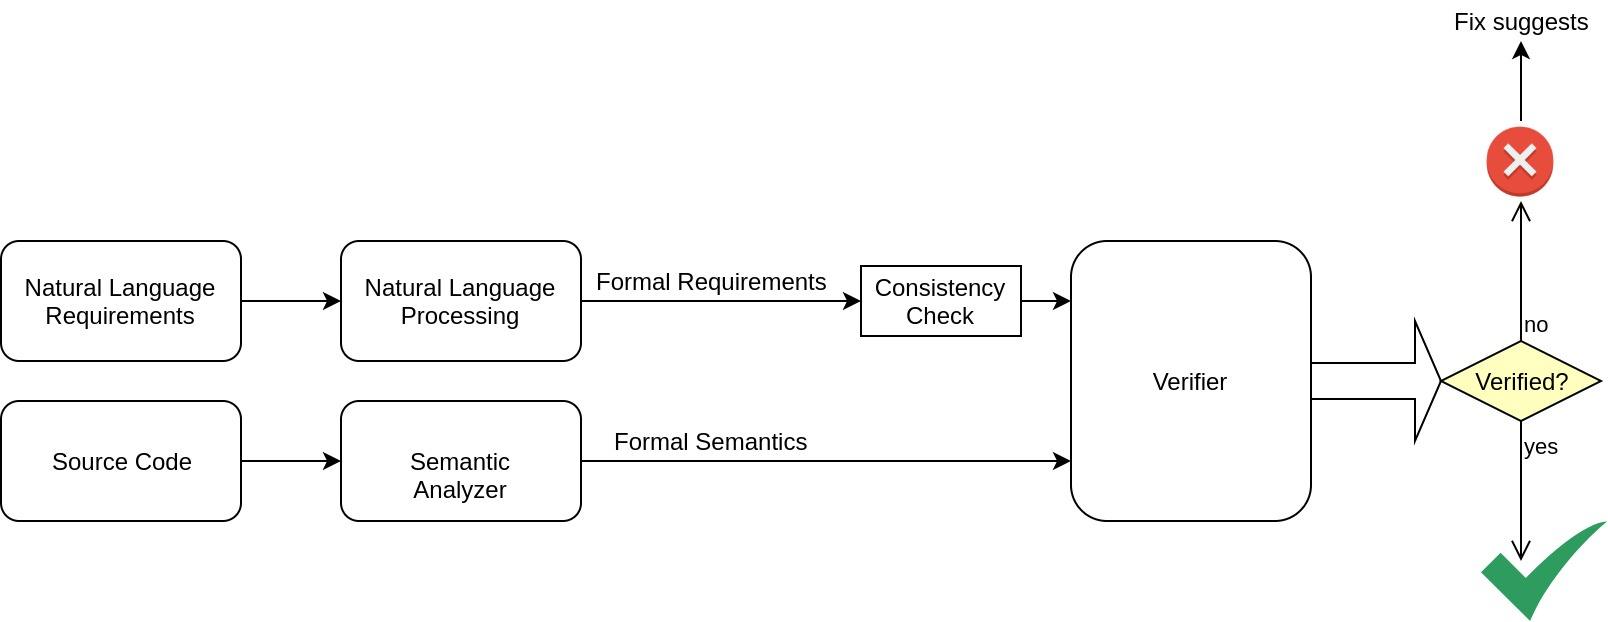
\includegraphics[width=1\linewidth]{Architecture}
	\caption[PorjArch]{Project Architecture}
	\label{fig:architectture}
\end{figure}


\gls{NLP} is used for formalizing the \gls{SRS}. Since, natural language is widely understood by stakeholders, it is used as a common way for representing requirements. Representing requirements in natural language suffers from potential problems like ambiguity, inconsistency and incompleteness. A systematic literature review in the last two decades from 1995 till 2016 shows that collecting ambiguous requirements is one of the highest critical challenges in software engineering \cite{Besrour}. Since the advent of software engineering, researchers used formal and semi-formal methods to overcome this problem. However, even when formal and semi-formal languages are used, there is no escape from natural language as the initial requirements are written in natural language \cite{Kamsties}. The consequences of ambiguous requirements will lead to excessive efforts, high cost and failure in some software projects. For example, software developers might decide a subjective interpretation of requirements based on their point of view. Ferrari et al. (2014) argued that this subjective interpretation leads to designing software in a different way from what was intended in the requirements \cite{Ferrari}. For several decades, \gls{SRS} processing and analysis has been the focus of research in software engineering discipline. Since natural language is ambiguous, a computer cannot provide full support to analyze \gls{SRS} in an automatic fashion. Consequently, the analysis of \gls{SRS} is conducted manually which consumes time, effort and cost. Most importantly, the manual analysis of requirements results in inefficiency and imprecise results \cite{Wang}. The problem will be more obvious and critical when software projects involve thousands of requirements and hundreds of \gls{SRS} documents. Conducting verification of thousands of requirements via humans will become extremely expensive \cite{Fanmuy}. Generally, the primary source of problems in requirement engineering is reliance on humans extensively \cite{Ahmed}. This discussion leads to the importance of finding an automatic way for processing \gls{SRS}. \gls{NLP} was used as a possible solution to resolve ambiguity and to provide valuable information to the intended software developers. Ryan (1993) argued that: ”It is highly questionable that the resulting system from \gls{NLP} would be of great use in requirements engineering” \cite{Ryan}. Nazir et al. (2017) conducted a systematic literature review on \gls{NLP} applications for software requirement engineering, he concluded that: “Manual operations are still required on initial plain text of software requirements before applying the desired \gls{NLP} techniques” \cite{Nazir}.

On the other hand the formal semantics of the source code is needed.  A formal semantics should serve as a solid foundation for any programming language development, so it must be correct and complete (to be trusted and useful), executable (to yield a reference implementation), and appropriate for program reasoning and verification.

The five most popular programming languages according to GitHub in 2019 is JavaScript, Python, Java, PHP and C\#. Several efforts to give JavaScript a formal semantics have been made, most notably by Politz et al. \cite{Politz} and Bodin et al. \cite{Bodin}. But Unfortunately, these address fragments of the language and are not fully validated with a formal JavaScript semantics. Having to define two or more different semantics for a real-life language, together with proofs of equivalence, is a huge burden in itself, not to mention that these all need to be maintained as the language evolves. Due to the functional nature of their interpreters, these semantics cannot handle the nondeterminism of JavaScript well. Finally, their interpreters are not suited for symbolic execution, and thus for developing program reasoning tools.


\bibliography{project_summary}{}
\bibliographystyle{plain}

\newpage

\section{List of Beneficiaries}


\begin{table}[hbpt]\centering
	\begin{adjustbox}{width=1\textwidth}
		\begin{tabular}{ |c|c|c|c|c|c|c|c|} 
			\hline
			\textbf{Beneficiary} & \textbf{Beneficiary} & \textbf{Beneficiary} & \textbf{Beneficiary} & \textbf{Country} & \textbf{Date enter} & \textbf{Date exit} \\
			\textbf{Number} & \textbf{name} & \textbf{short name} & \textbf{type} & ~ & \textbf{project} & \textbf{project} \\
			\hline
			
			1 & Eötvös Loránd & ELTE & RTD & Hungary & 2019.12.01 & 2022.12.01 \\
			(coordinator) & University & ~ & Performer & ~ & ~ & ~ \\
			\hline
			
			2 & Aalto & Aalto & RTD  & Finland & 2019.12.01 & 2022.12.01 \\
			~ & University & ~ & Performer & ~ & ~ & ~ \\
			\hline
			
			3 & Royal Institute & KTH & RTD  & Sweden & 2019.12.01 & 2022.12.01 \\
			~ & of Technology &  ~ & Performer & ~ & ~ & ~ \\
			\hline
			
			4 & Technical & TUB & RTD  & Germany & 2019.12.01 & 2022.12.01 \\
			~ & University Berlin &  ~ & Performer & ~ & ~ & ~ \\
			\hline
			
			5 & Université & UCA & RTD  & France & 2019.12.01 & 2022.12.01 \\
			~ & Côte d’Azur &  ~ & Performer & ~ & ~ & ~ \\
			\hline
			
			6 & University & UNITN & RTD  & Italy & 2019.12.01 & 2022.12.01 \\
			~ & of Trento &  ~ & Performer & ~ & ~ & ~ \\
			\hline
			
			7 & Elte-Soft & ~ & SME  & Hungary & 2019.12.01 & 2022.12.01 \\
			~ & Nonprofit Kft. &  ~ & Association & ~ & ~ & ~ \\
			\hline
			
			8 & Polarion & ~ & SME  & Germany & 2019.12.01 & 2022.12.01 \\
			~ & Software &  ~ & Association & ~ & ~ & ~ \\
			\hline
			
			9 & Rational & ~ & SME & United & 2019.12.01 & 2022.12.01 \\
			~ & Software &  ~ & Association & States & ~ & ~ \\
			\hline
		\end{tabular}
	\end{adjustbox}
	\caption{Table of Beneficiaries}
\end{table}


\section{The budget brakedown\footnote{All costs are in EUR}}

\begin{table}[hbpt]\centering
	\begin{adjustbox}{width=1\textwidth}
		\begin{tabular}{ |c|c|c|c|c|c|c|c|c|c|c|c|} 
			\hline
			\textbf{Participant} & \textbf{Organisation} & \textbf{Type} & \textbf{Funding} & \textbf{Indirect} & \textbf{RTD /} & ~ & ~ & ~ & \textbf{~} & \textbf{Total} & \textbf{Requested}\\
			
			\textbf{number in} & \textbf{short name} & ~ & \% & \textbf{costs} & \textbf{Innovation} & \textbf{Demonstration} & \textbf{Management} & \textbf{Other} & \textbf{Total} & \textbf{receipts} & \textbf{EU} \\
			
			\textbf{this project} & ~ & ~ & ~ & ~ & \textbf{(A)} & \textbf{(B)} & \textbf{(C)} & \textbf{(D)} & \textbf{(A+B+C+D)} & ~ & \textbf{contribution} \\
			
			~ & ~ & ~ & ~ & ~ & \textbf{costs} & \textbf{costs} & \textbf{costs} & \textbf{costs} & ~ & ~ & ~ \\
			\hline
			
			1 & ELTE & RTD & 71.43\% & 50.000 & 80.000 & 5.000 & 50.000 & 25.000 & 160.000 & 210.000 & 150.000 \\
			~ & ~ & Performer & ~ & ~ & ~ & ~ & ~ & ~ & ~ & ~ & \\
			\hline
			
			2 & Aalto & RTD & 63.89\% & 100.000 & 170.000 & 6.000 & 26.000 & 11.000 & 213.000 & 313.000 & 200.000 \\
			~ & ~ & Performer & ~ & ~ & ~ & ~ & ~ & ~ & ~ & ~ & \\
			\hline
			
			3 & KTH & RTD & 55.55\% & 110.000 & 200.000 & 13.000 & 30.000 & 7.000 & 250.000 & 360.000 & 200.000 \\
			~ & ~ & Performer & ~ & ~ & ~ & ~ & ~ & ~ & ~ & ~ &\\
			\hline
			
			4 & TUB & RTD & 55.55\% & 100.000 & 220.000 & 16.000 & 33.000 & 27.000 & 296.000 & 396.000 & 220.000 \\
			~ & ~ & Performer & ~ & ~ & ~ & ~ & ~ & ~ & ~ & ~ & \\
			\hline
			
			5 & UCA & RTD & 62.5\% & 80.000 & 120.000 & 12.000 & 20.000 & 8.000 & 160.000 & 240.000 & 150.000 \\
			~ & ~ & Performer & ~ & ~ & ~ & ~ & ~ & ~ & ~ & ~ & \\
			\hline
			
			6 & UNITN & RTD & 67.19\% & 75.000 & 120.000 & 20.000 & 25.000 & 13.000 & 178.000 & 253.000 & 170.000 \\
			~ & ~ & Performer & ~ & ~ & ~ & ~ & ~ & ~ & ~ & ~ & \\
			\hline
			
			7 & Elte-Soft & SME & 37.03\% & 50.000 & 70.000 & 5.000 & 10.000 & - & 85.000 & 135.000 & 50.000 \\
			~ & ~ & Association & ~ & ~ & ~ & ~ & ~ & ~ & ~ & ~ & \\
			\hline
			
			8 & Polarion & SME & 0.00\% & 90.000 & 20.000 & 2.000 & 10.000 & - & 32.000 & 122.000 & - \\
			~ & Software & Association & ~ & ~ & ~ & ~ & ~ & ~ & ~ & ~ & \\
			\hline
			
			9 & Rational & SME & 0.00\% & 25.000 & 5.000 & 10.000 & 15.000 & 4.000 & 34.000 & 59.000 & - \\
			~ & Software & Association & ~ & ~ & ~ & ~ & ~ & ~ & ~ & ~ & \\
			\hline\hline\Large
			\textbf{Total} &  &  & 54.6\% & 680.000 & 1.005.000 & 89.000 & 219.000 & 95.000 & 1.408.000 &\Large\textbf{2.088.000} &\Large\textbf{1.140.000}
			\\\hline
		\end{tabular}
	\end{adjustbox}
\caption{Table of Costs}
\end{table}


\newpage

\begin{center}
	\begin{adjustbox}{width=1\textwidth}
			\begin{tabular}{ |c|c|c|c|c|c|c|c|} 
			\hline
			\textbf{WP} & \textbf{WP Title} & \textbf{Type of} & \textbf{Lead} & \textbf{Person-} & \textbf{Start} & \textbf{End} \\
			\textbf{Number} & \textbf{~} & \textbf{activity} & \textbf{beneficiary} & \textbf{month} & \textbf{month} & \textbf{month}  \\
			~ & ~ & ~ & \textbf{number} & ~ & ~ & ~ \\
			\hline
			
			WP1 & Project Management & MGT & 1 & 18 & 1 & 36 \\
			\hline
			
			WP2 & Module definitions & RTD & 1 & 15 & 1 & 3\\
			\hline
			
			WP3 & NLP for Requirements Analysis& RTD & 4 & 36 & 4 & 13\\
			\hline
			
			WP4 & Semantic Analyzer & RTD & 3 & 48 & 4 & 16\\
			\hline
			
			WP5 & Consistency check & RTD & 5 & 30 & 12 & 18\\
			\hline
			
			WP6 & Verifier & RTD & 2 & 120 & 18 & 30\\
			\hline
			
			WP7 & Code fix suggestion & RTD & 6 & 36 & 30 & 36\\
			\hline
			
			WP8 & Lessons learned & OTHER & 1 & 4 & 1 & 36\\
			\hline
			
			WP9 & Demonstration & DEM & 1 & 4 & 1 & 36\\
			\hline
			\hline
			
			Total: ~ & ~ & ~ & ~ & 311 & ~ &	\\
			\hline
		\end{tabular}
	\end{adjustbox}
\end{center}

\newpage

\section{List of Deliverables}

\begin{table}[hbpt]\centering
	\begin{adjustbox}{width=1\textwidth}
			\begin{tabular}{ |c|c|c|c|c|c|} 
			\hline
			\textbf{Del.} & \textbf{Deliverable Title} & \textbf{WP} & \textbf{Nature} & \textbf{Dissemi-} & \textbf{Delivery} \\
			\textbf{no.} & \textbf{~} & \textbf{no.} & ~ & \textbf{nation} & \textbf{date}  \\
			~ & ~ & ~ & ~ & \textbf{level} & ~  \\
			\hline
			
			D1.1 & First Annual Report & 1 & R & PU & 12\\
			\hline
			
			D1.2 & Second Annual Report & 1 & R & PU & 24\\
			\hline
			
			D1.3 & Final Project Report & 1 & R & PU & 36\\
			\hline
			
			D2.1 & Module Specification & 2 & O & CO & 3\\
			\hline
			
			D3.1 & First NLP Prototype & 3 & P & C0 & 7\\
			\hline
			
			D3.2 & Final NLP Prototype & 3 & P & C0 & 13\\
			\hline
			
			D3.3 & NLP Project Paper & 3 & O & PU & 13\\
			\hline
			
			D4.1 & First Semantic Analyzer Prototype & 4 & P & C0 & 8\\
			\hline
			
			D4.2 & Final Semantic Analyzer Prototype & 4 & P & C0 & 16\\
			\hline
			
			D4.3 & Semantic Analyzer Project Paper & 4 & O & PU & 16\\
			\hline
			
			D5.1 & Consistency Check Prototype & 5 & P & C0 & 18\\
			\hline
			
			D6.1 & First Verifier Prototype & 6 & P & C0 & 24\\
			\hline
			
			D6.2 & Final Verifier Prototype & 6 & P & C0 & 30\\
			\hline
			
			D6.3 & Verifier Project Paper & 6 & O & PU & 13\\
			\hline
			
			D7.1 & Code Fix Suggester Prototype & 7 & P & C0 & 36\\
			\hline
			
			D8.1 & NLP Lessons Learned Report & 8 & P & PP & 14\\
			\hline
			
			D8.2 & Semantic Analyzer Lessons Learned Report & 8 & P & PP & 17\\
			\hline
			
			D8.3 & Verifier Lessons Learned Report & 8 & P & PP & 31\\
			\hline
			
			D8.4 & Final Lessons Learned Report & 8 & R & PP & 36\\
			\hline
			
			D9.1 & First Annual Demonstration & 9 & D & PU & 12\\
			\hline
			
			D9.2 & Participation in FM 2021 Conference & 9 & D & PU & 16\\
			\hline
			
			D9.3 & Second Annual Demonstration & 9 & R & D & 24\\
			\hline
			
			D9.4 & Final Project Demonstration & 9 & R & D & 36\\
			\hline
			
		\end{tabular}
	\end{adjustbox}
\caption{Table of Deliverables}
\end{table}

\newpage

\section{Work Package Descriptions}

\subsection{Work Package 1}

\begin{table}[hbpt]\centering
	\begin{tabular}{|p{0.35\linewidth}|p{0.06\linewidth}|p{0.06\linewidth}|p{0.06\linewidth}|
                     p{0.06\linewidth}|p{0.06\linewidth}|p{0.06\linewidth}|p{0.06\linewidth}|}\hline
		 Work package number& WP1 &
		 \multicolumn{4}{|c|}{Start date or starting event:}{}&
		 \multicolumn{2}{|c|}{                        1  }{}\\\hline
		 Work package title&\multicolumn{7}{|c|}{ Project Management }{}\\\hline
		 Activity Type&\multicolumn{7}{|c|}{ MGT }{}\\\hline
		 Participant number & 1 & 7 & 8 & 9 & ~ & ~ & ~ \\\hline
		 Person-months per participant: & 9 & 3 & 3 & 3 & ~ & ~ & ~ \\\hline
	\end{tabular}
\end{table}

\subsubsection{Objectives}
\begin{itemize}
	\item O1.1 Meet Project Deadlines: The management aims for keeping the project on track and meet the deadlines. To achieve this, state of the art project management tools will be used such as \gls{RTC}. The Universities will be overseen by ELTE while the companies manage themselves. 
	
	\item O1.2 Manage Necessary Deliverables: The management aims for reporting annually a clear view over the project for supervisory authorities.  
\end{itemize}

\subsubsection{Description of work}
\begin{itemize}
	\item O1.1 Meet the Project Deadlines
	\begin{itemize}
		\item T1.1.1: Bi-weekly management meetings should be hold between the project participants and the meeting minutes should be stored at a central location accessible by all stakeholders.
		\item T1.1.2: Up-to-date reports should be available and presented at the stakeholder meetings. 
	\end{itemize}
	\item O1.2 Manage Necessary Deliverables:
	\begin{itemize}
		\item T1.2.1: The management should create and present the First Annual Report to the supervisory authorities.   
		\item T1.2.2: The management should create and present the Second Annual Report to the supervisory authorities.
		\item T1.2.3: The management should create and present the Final Annual Report to the supervisory authorities.
	\end{itemize} 
\end{itemize}

\subsubsection{Deliverables}

\begin{itemize}
	\item D1.1 First Annual Report: It should contain the work done during the first year and the achievements while introducing the time plan of next year. The report should be easily understandable for the authorities and should cover all fields of work.
	\item D1.2 Second Annual Report: It should contain the work done during the first year and the achievements while introducing the time plan of next year. The report should be easily understandable for the authorities and should cover all fields of work.  
	\item D1.3 Final Project Report:  It should contain the work done during the whole project life cycle and the achievements. The report should be easily understandable for the authorities and should cover all fields of work.  
\end{itemize}



\printglossaries

\section{}



\end{document}
